%%%%%%%%%%%%%%%%%%%%%%%%%%%%%%%%%%%%%%%%%%%%%%%%
% chapter4.tex                                 %
% Contains formatting and content of chapter 4 %
%%%%%%%%%%%%%%%%%%%%%%%%%%%%%%%%%%%%%%%%%%%%%%%%
\chapter{Results}


\section{Numerical Results}

\noindent Implementation of the particle swarm optimization algorithm provides a way to solve
for the optimal orbital transfer between two concentric circular orbits. Table (\ref{tab:Numerical-Results}) shows
the results of these computations. The ratio $(\frac{m_f}{m_{0}})_h$ represents the final to initial mass
ratio for a Hohmann transfer between orbits, whereas $\frac{m_f}{m_0}$ is the mass ratio of the algorithm 
determined optimal solution.


\begin{table}[H]
  \centering
  \begin{tabular}{@{}lllllll@{}}
  \toprule
  $\beta$ & $\Delta t_1$ & $\Delta t_{co}$ & $\Delta t_2$ & $J$ & $m_f/m_0$ & $(m_f/m_0)_h$ \\ \midrule
  2 & 0.671 & 5.229 & 0.411 & 1.082 & 0.567062 & 0.56614 \\
  4 & 1.044 & 11.834 & 0.442 & 1.487 & 0.405365 & 0.407642 \\
  6 & 1.178 & 20.006 & 0.413 & 1.59 & 0.3638 & 0.368367 \\
  8 & 1.25 & 24.87 & 0.403 & 1.652 & 0.339164 & 0.353299 \\
  10 & 1.282 & 41.08 & 0.365 & 1.647 & 0.34106 & 0.346603 \\ \bottomrule
  \end{tabular}
  \caption{Numerical results for the optimum orbital transfer for different $\beta$ values }
  \label{tab:Numerical-Results}
  \end{table}

\noindent For all values of $\beta$ in Table (\ref{tab:Numerical-Results}) the computed final to initial mass ratio is similar to the final to 
initial mass ratio for a Hohmann transfer. For $\beta = 2$, this value exceeds its Hohmann
counterpart. This indicates this algorithm is effective in determining optimal orbit trajectories, without
requiring the impulsive thrust assumption as made in the Hohmann transfer calculations.

\begin{figure}[H]
    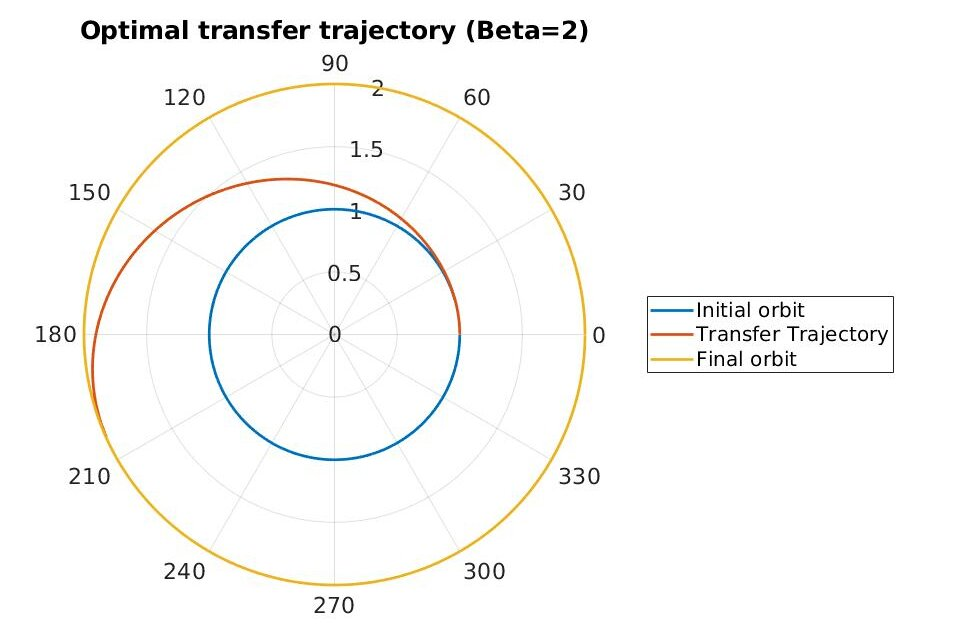
\includegraphics[width=\linewidth]{./jpgs/thrustArcB2.jpg}
    \caption{Numerically computed optimal transfer trajectory, $\beta = 2$.}
    \label{fig:Tarc-B2}
  \end{figure}

\noindent Fig. (\ref{fig:Tarc-B2}) displays the numerically computed optimal transfer
trajectory for $\beta = 2$. This yields insight into the optimal shape of the transfer orbit; a low 
eccentricity, relatively short orbital path connects the $R_2 = 2 LU$ and $R_1 = 1 LU$ circular orbits.

  \begin{figure}[H]
    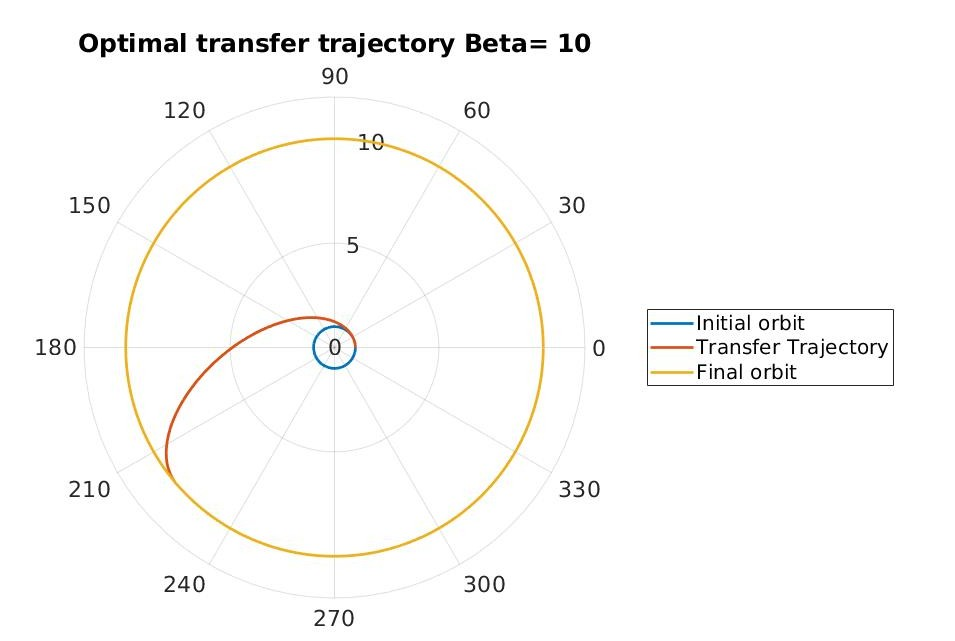
\includegraphics[width=\linewidth]{./jpgs/thrustArcB10.jpg}
    \caption{Numerically computed optimal transfer trajectory, $\beta = 10$.}
    \label{fig:Tarc-B10}
  \end{figure}

\noindent Analyzing Fig. (\ref{fig:Tarc-B10}) shows how the transfer orbit trajectory differs between two orbits 
with higher $\beta = \frac{R_2}{R_1}$ values. In comparison to Fig. (\ref{fig:Tarc-B2}), the transfer trajectory has
a much higher eccentricity and longer duration. In can thus be graphically and logically inferred that transfers between orbits 
with increasingly larger $\beta$ values are increasingly elliptical.

\begin{figure}[H]
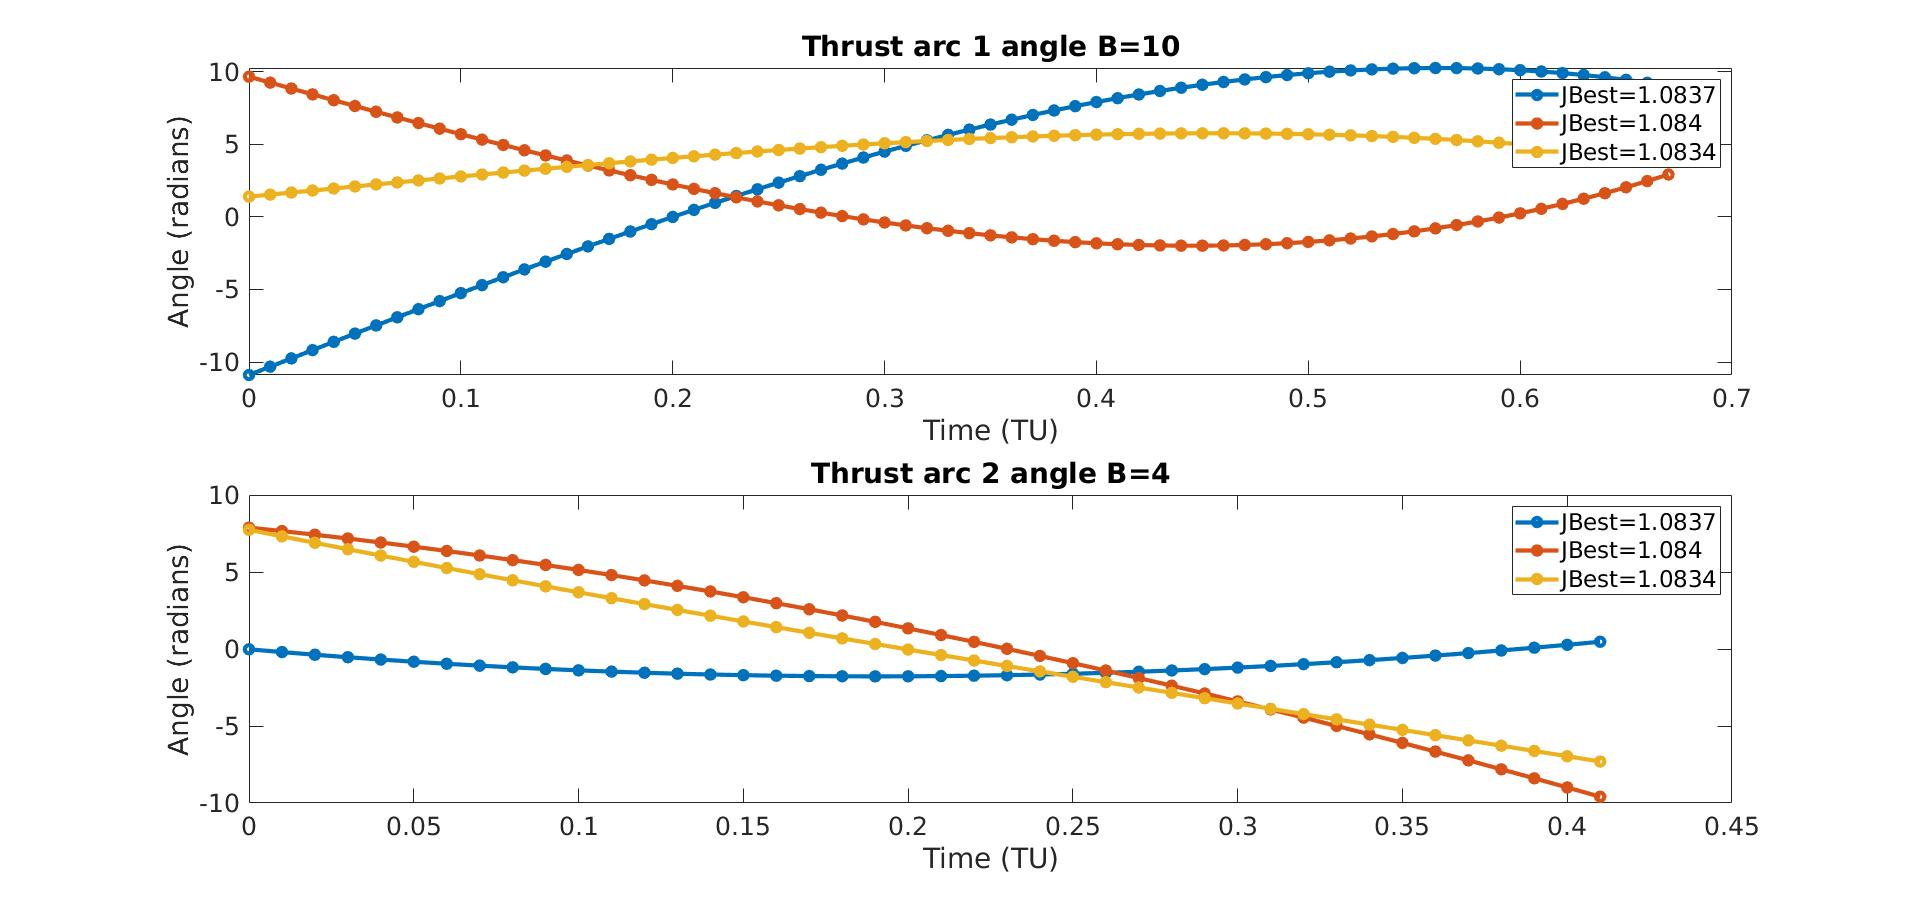
\includegraphics[width=\linewidth]{./jpgs/thrustAnglesB2.jpg}
\caption{Numerically computed thrust-angle time histories for optimal $\beta$ = 2 solutions  }
\label{fig:thrustAnglesB2}
\end{figure}

\noindent Particle swarm optimization's stochastic nature does not guarantee optimal results every 
run, nor does it guarantee that particles with similar cost function values represent similar solutions. 
Fig. (\ref{fig:thrustAnglesB2}) shows the thrust-pointing-angle time histories for both thrust arcs for 
different particles with quasi-optimal cost function values. While similar in cost function value, the 
thrust-pointing-angle histories vary greatly for these parameter sets. Thus, it can be observed that, within a search 
space of 11 unknowns, near optimal solutions may vary greatly in their characteristics.

\begin{figure}[H]
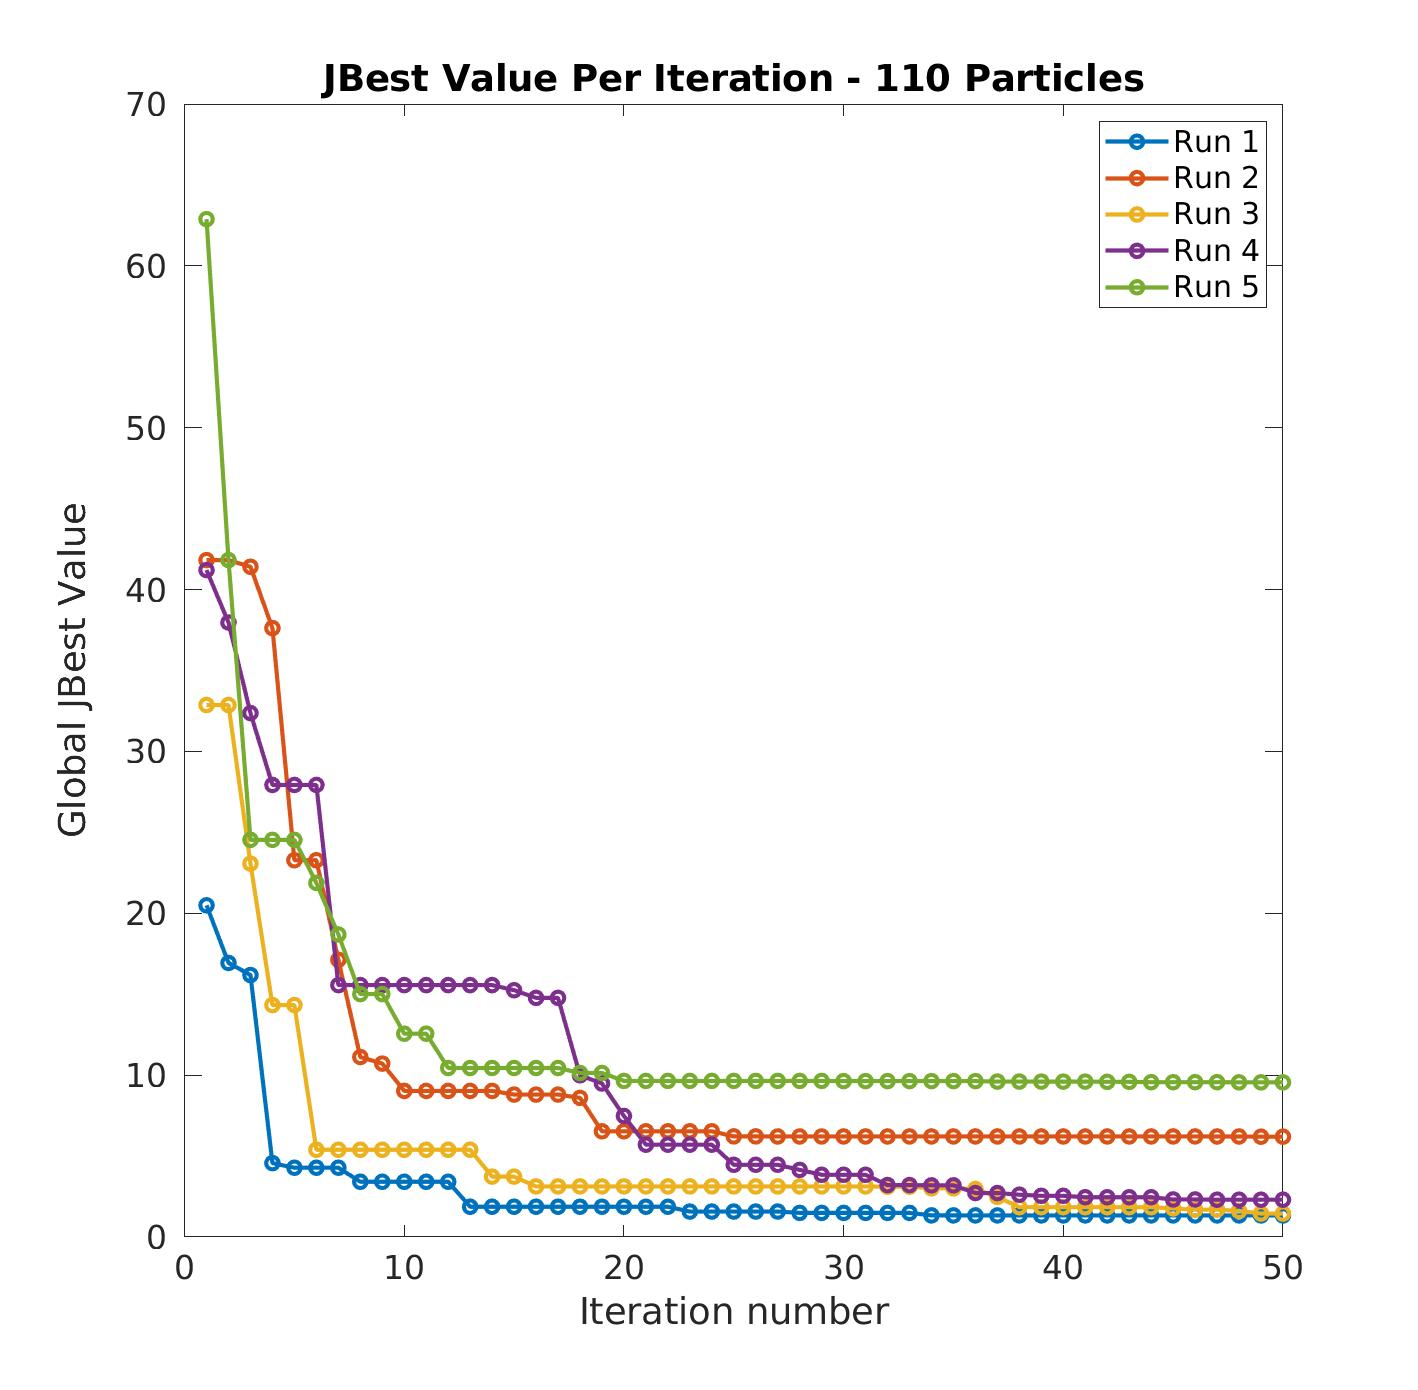
\includegraphics[width=\linewidth, height=13.5cm]{./jpgs/i50.jpg}
\caption{Global Best J Value Per Iteration: 100 Particles over 50 iterations}
\label{fig:gBestPer50Iter}
\end{figure}

\noindent Fig. (\ref{fig:gBestPer50Iter}) demonstrates the evolution of the best solution
found throughout the first 50 iterations of the algorithm. Two key results can be ascertained 
through this plot: First, the lowest found cost function value decreases rapidly over the first few
iterations. Second, the swarm may appear to stagnate at a cost function value then make a jump to a
better solution. This notion makes it difficult to discern when a population has truly stagnated. 

\begin{figure}[H]
    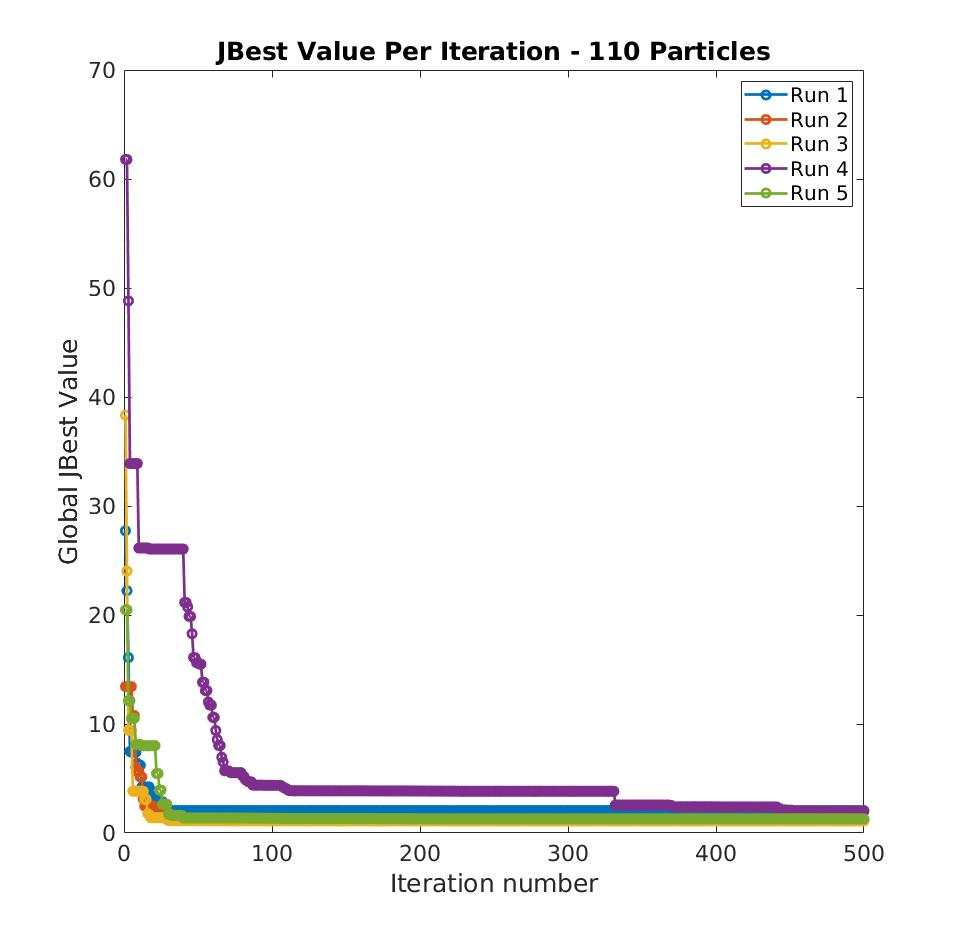
\includegraphics[width=\linewidth, height=13.5cm]{./jpgs/i500.jpg}
    \caption{Global Best J Value Per Iteration: 110 Particles over 500 iterations}
    \label{fig:gBestPer500Iter}
    \end{figure}

\noindent Fig. (\ref{fig:gBestPer500Iter}) showcases the evolution of global best cost function values over a larger 
range of iterations. This figure reinforces the observations from fig. (\ref{fig:gBestPer500Iter}). The rapid decrease 
in cost function value is generally limited to the beginning iterations, and cost function value
plateaus in the later stages of the algorithm. One notable portion is the significant decrease in the global best 
value for run four following over 300 iterations. This event demonstrates the inherent randomness of the particle swarm 
optimization algorithm, and once again illustrates how population stagnation can be difficult to predict.

\section{Rehydration Results}

\noindent \textit{Rehydration} is a method proposed within this thesis that resets a portion of the swarm if the population is estimated to 
be stagnated. This method is designed to inject more randomness into the population to explore more of the solution search space, 
i.e. \textit{rehydrate}, while
simultaneously exploiting previously computed knowledge of the solution set.

\noindent Results within this section are derived from the variation of the three main \textit{rehydration} parameters: $\delta_{Jcrit}$, $\eta_{iter}$,
and $P_{r,\text{\%}}$. Data from each combination of these parameters are presented.
The quantity $\bar{J}_{best}$ represents the average cost function value of 30 runs with the specified \textit{rehydration} 
parameters. The quantity $\Delta \bar{J}_{best,\text{\%}}$ is a measure of the percent change of $\bar{J}_{best}$ with \textit{rehydration} compared to 300 
runs of the same $P_{num}$ and $I_{num}$ without the reset method.



\begin{table}[H]
  \centering
  \begin{tabular}{lll|ll|ll}
    \toprule
    \multirow{2}{*}{$P_{r,\text{\%}}$ = 25} &
      \multicolumn{2}{c}{$\delta_{Jcrit} = .1\%$  } &
      \multicolumn{2}{c}{$\delta_{Jcrit} =  1\%$} &
      \multicolumn{2}{c}{$\delta_{Jcrit} = 5\%$} \\
      \cmidrule{2-7}
    & $\bar{J}_{best}$ & $\Delta \bar{J}_{best,\text{\%}}$ & $\bar{J}_{best}$ & $\Delta \bar{J}_{best,\text{\%}}$ & $\bar{J}_{best}$ & $\Delta \bar{J}_{best,\text{\%}}$ \\
    \midrule

    $n_{iter}=5$ & 1.347 & 44.177\% & 1.54 & 36.179\% & 1.438 & 40.406\% \\
    $n_{iter}=10$ & 1.421 & 41.11\% & 1.379 & 42.851\% & 1.594 & 33.941\% \\
    $n_{iter}=20$ & 1.331 & 44.840\% & 1.652 & 31.538\% & 1.503 & 37.712\% \\
    \bottomrule
  \end{tabular}
  \caption{Rehydration results for a 25\% population reset}
  \label{tab:rehydation-p25}
\end{table}

\noindent Table (\ref{tab:rehydation-p25}) shows the \textit{rehydration} results with $P_{r,\text{\%}}$ held constant
at $25\%$. Every combination of parameters produces a major improvement over the standard particle swarm optimization algorithm,
with percent improvement ranging from 31 to over 44 percent. In general, it can be observed that parameter sets 
with lower values of $\delta_{Jcrit}$ perform better. 

\begin{table}[H]
  \centering
  \begin{tabular}{lll|ll|ll}
    \toprule
    \multirow{2}{*}{$P_{r,\text{\%}}$ = 33} &
      \multicolumn{2}{c}{$\delta_{Jcrit} = .1\%$ } &
      \multicolumn{2}{c}{$\delta_{Jcrit} = 1\%$ } &
      \multicolumn{2}{c}{$\delta_{Jcrit} = 5\%$ } \\
      \cmidrule{2-7}
    & $\bar{J}_{best}$ & $\Delta \bar{J}_{best,\text{\%}}$ & $\bar{J}_{best}$ & $\Delta \bar{J}_{best,\text{\%}}$ & $\bar{J}_{best}$ & $\Delta \bar{J}_{best,\text{\%}}$ \\
    \midrule

    $n_{iter}=5$ & 1.371 & 43.18\% & 1.475 & 38.872\% & 1.412 & 41.484\% \\
    $n_{iter}=10$ & 1.364 & 43.47\% & 1.558 & 35.433\% & 1.473 & 40.448\% \\
    $n_{iter}=20$ & 1.412 & 41.48\% & 1.531 & 36.552\% & 1.578 & 34.604\% \\
    \bottomrule
  \end{tabular}
  \caption{Rehydration results for a 33\% population reset}
  \label{tab:rehydation-p33}
\end{table}

\noindent Data from Table (\ref{tab:rehydation-p33}) displays results with $P_{r,\text{\%}}$ set to 33\%. These data indicate similarly
improved algorithm performance for any parameter combination. However, just as in Table (\ref{tab:rehydation-p25}), the best results
originate from parameter combinations with $\delta_{Jcrit} = .1$.

\begin{table}[H]
    \centering
    \begin{tabular}{lll|ll|ll}
      \toprule
      \multirow{2}{*}{$P_{r,\text{\%}} = 50$} &
        \multicolumn{2}{c}{$\delta_{Jcrit} = .1\%$ } &
        \multicolumn{2}{c}{$\delta_{Jcrit} = 1\%$ } &
        \multicolumn{2}{c}{$\delta_{Jcrit} = 5\%$ } \\
        \cmidrule{2-7}
      & $\bar{J}_{best}$ & $\Delta \bar{J}_{best,\text{\%}}$ & $\bar{J}_{best}$ & $\Delta \bar{J}_{best,\text{\%}}$ & $\bar{J}_{best}$ & $\Delta \bar{J}_{best,\text{\%}}$ \\
      \midrule

      $n_{iter}=5$ & 1.58 & 34.52\% & 1.469 & 39.12\% & 1.425 & 40.94\% \\
      $n_{iter}=10$ & 1.396 & 42.15\% & 1.306 & 45.88\% & 1.473 & 38.96\% \\
      $n_{iter}=20$ & 1.373 & 43.10\% & 1.39 & 42.40\% & 1.33 & 44.88\% \\
      \bottomrule
    \end{tabular}
    \caption{Rehydration results for a 50\% population reset}
    \label{tab:rehydation-p50}
  \end{table}

\noindent Table (\ref{tab:rehydation-p50}) showcases \textit{rehydration} performance with 
$P_{r,\text{\%}}$ maintained at 50\%. Once again, every combination of parameters leads to 
significant reduction in $\bar{J}_{best}$ relative to the \textit{non-rehydation} algorithm. 
Within these results it can be observed that higher values of
$\eta_{iter}$ give the best performance. Unlike Tables (\ref{tab:rehydation-p25}, \ref{tab:rehydation-p33}), 
the value of $\delta_{Jcrit}$ appears to be less correlated to algorithm improvement.

\section{Algorithm Benchmarking}

\noindent Evaluation of a candidate solution to the finite thrust transfer problem requires significant computational resources.
These potential solutions must be calculated for every particle throughout every iteration, leading to long algorithm execution cycles.
Additionally, the inherent randomness of particle swarm optimization algorithms require them to be ran multiple times in the
pursuit of a quasi-optimal solution. The combination of these factors prove execution time to be paramount, thus the benchmarking
analysis done within this section. \newline

\noindent To aid in the presentation of the benchmarking results the additional parameters $\eta_{su\%}$, $\eta_{su}$, and $\eta_{su,st\%}$ are defined. 
These quantities relate the speedup of different implementations to the base MATLAB version, with all parameters held constant. 
They are computed as

\begin{equation}
\eta_{su\%} = 100*\frac{\text{MATLAB Time} - \text{Execution Time}}{\text{MATLAB Time}}
\label{eq:etaSUpercent}
\end{equation}


\begin{equation}
  \eta_{su} = \frac{\text{MATLAB Time}}{\text{Execution Time}}
  \label{eq:etaSU}
  \end{equation}


\begin{equation}
  \eta_{su,st\%} = \frac{\text{C++ Single Threaded Time} - \text{Execution Time}}{\text{C++ Single Threaded Time}}
  \label{eq:etaSUSTpercent}
  \end{equation}

\noindent These parameters serve to yield an insight into how algorithm performance differs between implementations
with the variation of $P_{num}$ and $I_{num}$.

\subsection{MATLAB}


%Putting the H here ensures the table goes exactly where you put
%it in the code
\begin{table}[H]
    \centering
    \begin{tabular*}{.5\textwidth}{c @{\extracolsep{\fill}} cc}
    \toprule
    \bm{$P_{num}$} & \bm{$I_{num}$} & \textbf{Time (s)} \\ \midrule
    25                        & 250            & 30.527   \\
    25                        & 500            & 39.15    \\
    25                        & 1000           & 68.88    \\
    50                        & 250            & 30.527   \\
    50                        & 500            & 80.4246  \\
    50                        & 1000           & 141.151  \\
    100                      & 250            & 95.956   \\
    100                      & 500            & 152.22   \\
    100                      & 1000           & 306.732  \\
    150                      & 250            & 161.3    \\
    150                      & 500            & 195.87   \\
    150                      & 1000           & 388.03   \\
    200                      & 250            & 157.061  \\
    200                      & 500            & 251.575  \\
    200                      & 1000           & 457.55   \\ \bottomrule
    \end{tabular*}
    \caption{MATLAB Numerical Results - Wall Clock Time}
    \label{tab:MATLAB-speedup}
    \end{table}

\noindent Table (\ref{tab:MATLAB-speedup}) presents base MATLAB implementation data throughout the range of $P_{num}$ and $I_{num}$
to be benchmarked. Execution time increases rather linearly with iteration number, but scales slower as $P_{num}$ grows. Results within
this data set form the basis of the comparisons presented within Tables (\ref{tab:ST-speedup}, \ref{tab:OpenMP-speedup}).
  
\subsection{C++ Single Threaded}

% Please add the following required packages to your document preamble:
% \usepackage{booktabs}
\begin{table}[H]
    \centering
    \begin{tabular}{@{}lllll@{}}
    \toprule
    \bm{$P_{num}$} & \bm{$I_{num}$} & \textbf{Time (s)} & \bm{$n_{su\%}$} & \bm{$n_{su}$} \\ \midrule
    25          & 250  & 1.732    & 94.32633406          & 17.62528868              \\
    25          & 500 & 2.39     & 93.89527458          & 16.38075314              \\
    25          & 1000 & 3.92     & 94.30894309          & 17.57142857              \\
    50          & 250 & 2.96     & 90.30366561          & 10.31317568              \\
    50          & 500 & 3.26     & 95.94651388          & 24.6701227               \\
    50          & 1000 & 5.695    & 95.96531374          & 24.78507463              \\
    100         & 250 & 6.659    & 93.060361            & 14.40997147              \\
    100         & 500 & 7.21     & 95.2634345           & 21.11234397              \\
    100         & 1000 & 11.83    & 96.14321297          & 25.92831784              \\
    150         & 250 & 7.26     & 95.49907006          & 22.21763085              \\
    150         & 500 & 12.64    & 93.54674018          & 15.4960443               \\
    150         & 1000 & 16.68    & 95.7013633           & 23.26318945              \\
    200         & 250 & 7.77     & 95.05287754          & 20.21377091              \\
    200         & 500 & 11.423   & 95.45940574          & 22.02354898              \\
    200         & 1000 & 21.06    & 95.39722435          & 21.72602089              \\ \bottomrule
    \end{tabular}
    \caption{C++ Single Threaded Speedup Results - Wall Clock Time}
    \label{tab:ST-speedup}
    \end{table}

\noindent Data within Table (\ref{tab:ST-speedup}) illustrate how the single threaded C++ implementation of 
the particle swarm optimization algorithm compares to the MATLAB version. It is evident that the C++ version is
clearly more performant, topping out at 96.1\% greater efficiency and 29.1 times faster than its
MATLAB counterpart. An analysis of these results indicates that, in general, the improvement differential becomes 
greater as $I_{num}$ increases.

\subsection{C++ Parallelization}
\begin{table}[H]
    \centering
    \begin{tabular}{@{}llllll@{}}
    \toprule
    \bm{$P_{num}$} & \bm{$I_{num}$} & \textbf{Time (s)} & \bm{$n_{su\%}$} & \bm{$n_{su,st\%}$} & \bm{$n_{su}$} \\ \midrule
    25  & 250 & 1.78  & 94.16909621 & -2.771362587 & 17.15       \\
    25  & 500& 3.4   & 91.31545338 & -42.25941423 & 11.51470588 \\
    25  & 1000& 5.23  & 92.40708479 & -33.41836735 & 13.17017208 \\
    50  & 250 & 2.81  & 90.7950339  & 5.067567568  & 10.86370107 \\
    50  & 500& 4.77  & 94.06897889 & -46.3190184  & 16.86050314 \\
    50  & 1000& 8.51  & 93.9709956  & -49.42932397 & 16.58648649 \\
    100 & 250& 5.71  & 94.04935595 & 14.2513891   & 16.80490368 \\
    100 & 500& 6.6   & 95.66417028 & 8.460471567  & 23.06363636 \\
    100 & 100 & 11.73 & 96.17581472 & 0.8453085376 & 26.14936061 \\
    150 & 250 & 4.92  & 96.94978301 & 32.23140496  & 32.78455285 \\
    150 & 500 & 9.77  & 95.01199775 & 22.7056962   & 20.04810645 \\
    150 & 1000& 13.93 & 96.41007139 & 16.48681055  & 27.85570711 \\
    200 & 250 & 5.88  & 96.25623166 & 24.32432432  & 26.71105442 \\
    200 & 500 & 10.46 & 95.84219418 & 8.4303598    & 24.05114723 \\
    200 & 1000 & 22.42 & 95.09998907 & -6.457739791 & 20.40811775 \\ \bottomrule
    \end{tabular}
    \caption{\code{OpenMP} Speedup Results - Wall Clock Execution Time}
    \label{tab:OpenMP-speedup}
    \end{table}

\noindent Table (\ref{tab:OpenMP-speedup}) displays the speedup of the \code{OpenMP} 
implementation relative to the base C++ and MATLAB versions. At peak efficiency, this implementation
achieves a 96.49\% speedup at 32.78 times faster than the MATLAB execution. However, under certain
conditions, the parallelized version of the algorithm is slower than the single threaded version. Analysis 
of the data suggests this occurs in cases with a lower $P_{num}$ and higher $I_{num}$. \newline

\noindent The reasoning for this
is likely two-fold: First, parallelization improves the algorithm during early iterations, where the numerical 
integrations for many particles of the population do not converge, requiring greater computation. In these 
instances, the improvements from parallelizing the particle evaluation step overcome the multi-threaded overhead
for the iteration. Throughout the later iterations of the algorithm, where most numerical integrations converge quickly,
the multi-threaded overhead outweighs the parallelization improvements. Second,
as $P_{num}$ decreases, so does the benefit arising from parallelizing particle evaluation. Thread setup
overhead, however, remains constant independent of $P_{num}$, leading to net decreased efficiency. One potential way 
to maintain increased efficiency throughout may be to parallelize the process in early iterations and run the algorithm
single threaded in later stages.

\newpage